\documentclass[USenglish]{ifimaster}  %% ... or USenglish or norsk or nynorsk
\usepackage[utf8]{inputenc}           %% ... or latin1
\usepackage[T1]{fontenc,url}
\usepackage{todonotes}
\urlstyle{sf}
\usepackage{babel,textcomp,csquotes,duomasterforside,varioref,graphicx}
\usepackage[backend=biber,style=numeric-comp]{biblatex}
\usepackage{acronym}
\usepackage{amsmath , amssymb , amsthm}
\usepackage[margin=1.5in, footskip=0.25in]{geometry}
%\setcounter{tocdepth}{5}

\title{Image-based terrain characterization for autonomous vehicles, based on deep learning}        %% ... or whatever

\author{Andreas Hagen}                      %% ... or whoever 

\bibliography{references.bib}                  %% ... or whatever



\begin{document}
\duoforside[dept={Department of Technology Systems},   %% ... or your department
  program={Cybernetics},  %% ... or your programme
  short]                                        %% ... or long

\frontmatter{}
\chapter*{Abstract}                   %% ... or Sammendrag or Samandrag

\tableofcontents{}
\listoffigures{}
\listoftables{}

\chapter*{Preface}
\chapter*{Abbreviations}
%\addcontentsline{toc}{chapter}{Abbreviations} \noindent
%--- Acronyms -----------------------------------------------------------------%
% \acrodef{label}[acronym]{written out form} % acronym syntax
%\acrodef{etacar}[$\eta$ Car]{Eta Carinae}   % acronym example
%--- Acronyms -----------------------------------------------------------------%
% how to use acronyms:
% \ac = use acronym, first time write both, full name and acronym
% \acf = use full name (text + acronym)
% \acs = only use acronym
% \acl = only use long text
% \acp, acfp, acsp, aclp = use plural form for acronym (append 's')
% \acsu, aclu = write + mark as used
% \acfi = write full name in italics and acronym in normal style
% \acused = mark acronym as used
% \acfip = full, emphasized, plural, used
%--- Acronyms -----------------------------------------------------------------%
\begin{acronym}
        \acro{ai}[AI]{artificial intelligence}
        \acro{ann}[ANN]{artificial neural networks}
        \acro{cnn}[CNN]{convolutional neural networks}
        \acro{dl}[DL]{deep learning}
        \acro{ml}[ML]{machine learning}
        \acro{cpu}[CPU]{central processing unit}
        \acro{gpu}[GPU]{graphics processing unit}
        \acro{gui}[GUI]{graphical user interface}
        \acro{rgb}[RGB]{red, green, blue}
\end{acronym}


\mainmatter{}
\chapter{Introduction}                  
\section{Motivation}
\section{Background}
\section{Problem description}
\section{Thesis outline}

\chapter{Theoretical background}
This chapter will begin providing an short overview of the basics of \ac{ai}, \ac{ml}, computer vision, and \acf{dl}. There is a \ac{dl} framework being used for implementing the network in the thesis, while a few computer vision techniques is being used for processing the images further after the predictions. The reasoning behind choosing \ac{dl} is shortly discussed. Further is the necessary data preprocessing described, before the basics of different \ac{ann} is covered. Lastly this section will go through the theory of generating ground truth labels with a suitable program.

\section{Artificial intelligence}
\ac{ai} is a field where machines are able to demonstrate intelligence through mathematics, statistics and logic. It has the ability to tackle many complex problems which are intellectually difficult or impossible to solve for a human being with natural intelligence. Even though \ac{ai} could solve complex problems, it still had a few challenges in the early days. Some intuitive tasks for us like recognize a cat or a dog in an image, or the context of a written text, proved to be a true challenge. A solution to these problems was to allow machines to learn from experience, which is where \ac{ml} and \ac{dl} comes into the picture \cite{The_holy_grail_of_DL}.

\begin{figure}[ht]
    \centering
    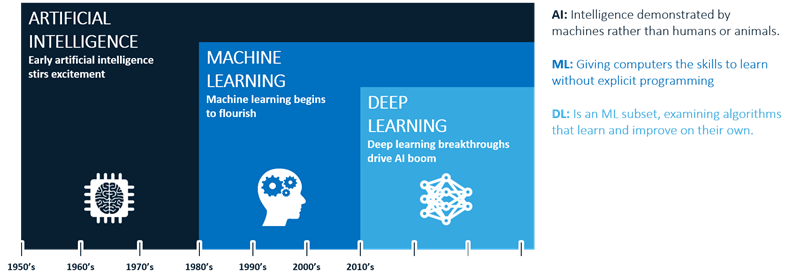
\includegraphics[width=0.8\textwidth]{bilder/AI_ML_DL.png}
    \caption{The provisional timeline for AI, ML, and DL \cite{website:AI}}
    \label{fig:AI}
\end{figure}

\subsection{Machine learning}
Figure \ref{fig:AI} illustrates that \ac{ml} is a subset from \ac{ai}. The term is further well defined by \ac{ml} pioneer Tom M. Mitchell:
\newline
\newline
\textit{“Machine learning is the study of computer algorithms that allow computer programs to automatically improve through experience.”} \cite{tom_mitchell}.
\newline
\newline
Instead of being explicitly programmed to improve their performance on a task like algorithms in \ac{ai}, \ac{ml} learns through experience. Even though \ac{ml} techniques is not used in this thesis, it is combined with \ac{ai} the foundation for \ac{dl}.

\subsection{Deep learning}
As visualized in figure \ref{fig:AI}, \ac{dl} is a subset of both \ac{ai} and \ac{ml}. The main difference between \ac{ml} and \ac{dl},  is that \ac{dl} is able to learn data representations from data sets instead. The whole network is in other words able to solve the problem from start to end without using external methods as in \ac{ml}. \ac{dl} has its networks (called \ac{ann}) loosely based on the same principle as the neuron system from a human brain. 

\subsubsection{Supervised learning}
Supervised learning is the most commonly used technique in \ac{dl} \cite{Francois_Deep_learning_with_python}. The word supervised refers to known targets or annotations in the form of a labelled data set. With that knowledge a function can learn how to map input data to the targets.

\subsection{Benefits using \ac{dl} with \ac{cnn} vs traditional methods}
\ac{dl} has been increasingly more popular during the last few years. Some of the reason for that has been its ability to provide higher accuracy when trained with large amounts of data. It tends also to provide better results in network with smaller data sets, as being the case in this thesis. This benefit over traditional methods alone would be enough to consider taking \ac{dl} as preferred method.
\newline
\newline
Another benefit using \ac{dl} over traditional methods is the features extraction from images. While the traditional algorithms needs to manually implement different computer vision techniques in order to extract the desired features before classification, this is not the case in \ac{dl}. With the use of convolution layers from \ac{cnn} the features are extracted automatically from the layers.
The first layer will detect and learn small edges. Then the second layer will learn larger patterns made from the features from the first layer, and this concept will repeat itself in the further layers. The patterns being learned are translation-invariant, which means it can recognize the learned pattern if it appears anywhere else in the image \cite{Francois_Deep_learning_with_python}. This advantage is exclusively for the \ac{cnn}, and make the networks able to generalize better with less training samples than other networks.

\section{Computer vision}
Computer vision is a field which main purpose is to make machines be able to interpret and understand features from images or video. In other words, "Teaching computers how to see"\cite{website:maskinsyn-intro}. This section will only go through a small number of computer vision concepts, as they are being used in the thesis.
\subsection{Semantic segmentation}
Segmentation is a concept where the input is in the form of an image, and the output consists of regions and structures based on the input. Normal segmentation will in most cases only provide a basic scene understanding. If we want to understand what is in the image more thoroughly, semantic segmentation is the next step. The idea behind semantic segmentation is that instead of regions, every pixel in the image gets classified. Which means there will be possible to gain a broader scene understanding of the environment in the image, making it easier to recognize different elements.
\subsection{Morphological operations}
A common binary image operations are called \textit{morphological operations}, since
they change the shape of the underlying binary objects \cite{Ritter}. This is done by convolving a binary \textit{structuring element} on the binary image, where the structuring element can be any chosen shape. These operations are typically used to clean up binary images, and two of the standard binary morphological operations used in the thesis are: 
\newline
\begin{itemize}
    \item \textbf{Erosion}
    \item \textbf{Dilation}
\end{itemize}

Where \textit{erosion} thins the object and \textit{dilation} thickens the object. Using these operations in this specific order (erosion + dilation) results in \textit{opening}. This operation tends to close large regions, smooth boundaries, while also removing some noise from the image. There is common to experiment how many iterations there should be implemented in each the erosion and the dilation operation.
\newline
\newline
The structuring element used is a normally a square rectangular kernel of desired size. It can also take the shape of an circle if necessary. This depends on what the regions in the image looks like. Sometimes a circle shaped kernel may be a better option to smooth the curves than the normal rectangular kernel.
\subsection{Connected component analysis}
The connected component analysis is a tool which can be used to filtering out noise from a predicted image. It labels all the connected regions in the image automatically in an iterative manner. That way it is possible to mask out every label which contains less pixels than a given threshold. If the region after the noise filtering contain holes surrounded by a complete polygon, these can be sealed with an binary object filler. If both operations is implemented successfully, the improvement from the original prediction will be significantly better.

\section{Data preprocessing}
This section will cover data processing from an image-based point of view. Before the data set can be fed into the network, would it in the most cases be inevitable to perform several preprocesses. This is necessary in order to make the data prepared for training. 
\newline
A common thing to do with an image-based data set is to resize the images to a slightly lower resolution. This is especially necessary if the computer does not have a state-of-art \ac{gpu}, as the model otherwise might be very slow. The down scaling will help the model to be more effective and less time consuming, at the prize of loosing some features from the original resolution. It is therefore important to test different scales, to find the perfect fit between keeping enough key features and have an effective model.
\newline
A \ac{rgb} image contains integer values in the range from 0-255 in each of its three channels. Because the values of the weights in a neural network is relatively small, it is normal practice to normalize the image-array to values between 0-1. This can be done by divide the array with 255. Doing so will prevent to slow down the learning process, as the values from the weights and the array now are in closer range. Casting the array from int to float before normalizing would increase the accuracy even further. This is due to the float division results in a more accurate number than int division.\todo{legg til bilde eller ligning med forklaring} 
\newline
\newline
Another process is to check whether the data set has the correct shape or not. This is necessary because the network needs to know which input shape to expect. The input layer in Keras is a tensor which are passed to the first hidden layer. If that input layer does not correspond with the shape of each element in the data set, the network will not be able to execute. In the case where "Conv2D" layers are used in a Keras framework, an input array needs to have the following structure:
\newline
\newline
(height, width, channels)
\newline
\newline
Where height and width refers to the x- and y-coordinates in the image, and channels refers to if the image is binary (channels=1) or \ac{rgb} (channels=3).
\subsection{Data augmentation}
Data augmentation is a helpful tool in order to maintain a more generalized model. It is a method for applying transformations to the training data. When the images are pre-processed with the methods described in this section, the network learns how to cope with slightly different images than the original training set. This is the reason the model have a higher chance of predicting the test images (images that the model never have seen before) with more accuracy. In addition to potentially higher accuracy, the model also has lower chance of overfitting. This sub-section will only cover the most used augmentation techniques.  
\subsubsection{Random cropping}
A popular method in augmentation is random cropping. Which means sampling a random chosen square box from the original image, and then resize to the original size.\todo{sett inn bilde} As seen in figure \todo{referer til bildet} the image focus on different areas from the original image, due to the random chosen box. This operation must be included with the ground truth images. When an operation changes the geometry in the image, the same operation must be done in the ground truth image in order to still be a valid target. 
\subsubsection{Flipping images}
Another method is to flip the images in either vertical or horizontal order. Even when the images are flipped, are they recognizable for the model. The ground truth must also go through the same operation in order to keep the correct geometry in both images. 
\subsubsection{Color changes}
The idea behind color changes is to make the the model more robust and generalized for new unseen data. Since the geometry in the images are the same after applying color changes, is it not necessary to do any operation on the ground truth images.
\section{Artificial neural networks}
Mostly of the theory in this section is based on the theory from the Stanford University course \textit{"CS231n: Convolutional Neural Networks for Visual Recognition"}\cite{website:cs231n}, and from the course \textit{"INF4490 – Biologically Inspired Computing"}\cite{website:inf_4490_slp}\cite{website:inf_4490_mlp} at University of Oslo.
\newline
\newline
An \ac{ann} is a computing system which is vaguely based on the same principle as biological neurons in a human brain. It has the ability to learn different tasks and data representations. To fully understand the concept, the basics of a neural network is divided into different parts and further described in this section.
\newline
\newline
\subsection{Single- and multi-layer neural network}
In 1943 McCulloch \& Pitts designed a much simplified version of biological neurons\cite{mcculloch_pitts}. With their design, they are widely known as the inventors of the first \ac{ann}. Their ideas of a threshold in the activation function and combining many basic units in order to increase computational power are still being used nowadays.
\begin{figure}[ht]
    \centering
    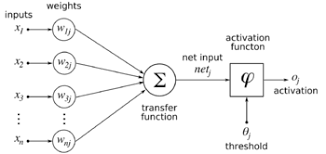
\includegraphics[width=0.8\textwidth]{bilder/mcculloch_and_pitts.png}
    \caption{Illustrates the McCulloch \& Pitts design of a simplified neuron \cite{website:mcCulloch_img}}
    \label{fig:mcculoch_and_pitts}
\end{figure}
The illustration of the neuron and its activation function in figure \ref{fig:mcculoch_and_pitts} can be mathematically explained with equation \ref{eq:mcCulloch}.
\begin{equation}\label{eq:mcCulloch}
\begin{aligned}
    {h = \sum_{i=1}^{n} x_i \omega_i \quad , \quad\quad o = 
\begin{cases}
    1 & \text{ h $\geq$ $\theta$ }  \\
    0 & \text{ h < $\theta$ }
\end{cases}}
\end{aligned}
\end{equation}
Where the neurons function ($h$) is denoted in the form of a dot product between the inputs ($x_i$) and the weights ($\omega_i$). The neurons activation function \textit{"fires"} when the dot product of the input and its weight respectively are higher than a given threshold $\theta$. Meaning the output ($o$) becomes 1 when $h$ is equal to or higher than the threshold, and 0 when $h$ is lower than the threshold value.
\newline
\newline
If many McCulloch \& Pitts neurons are put together, the structure of a single-layer neural network appears. A single-layer perceptron like that are able to learn linear problems. When the task is to learn non-linear problems, the solution is to add one or more hidden layers as done in multi-layer perceptron.   
\begin{figure}[ht]
    \centering
    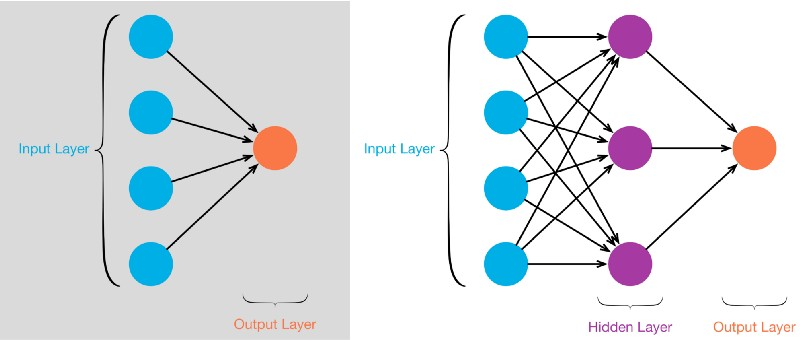
\includegraphics[width=0.8\textwidth]{bilder/slp_&_mlp.jpeg}
    \caption{Single-layer perceptron to the left, and multi-layer perceptron to the right \cite{website:slp_mlp}}
    \label{fig:slp_mlp}
\end{figure}
The difference can be seen visually by figure \ref{fig:slp_mlp}, where the single-layer perceptron only has an input and an output layer, while the multi-layer perceptron includes at least one hidden layer.
\newline
\newline
\subsection{The learning rule}
In order for the single-layer neural network to learn, it has to adjust the weights accordingly. This is were the perceptron learning rule comes into the picture.

\begin{equation}\label{eq:learning_rule}
\begin{aligned}
\omega_{ij} \longleftarrow \omega_{ij} + \Delta\omega_{ij}
\end{aligned}
\end{equation}
Equation \ref{eq:learning_rule} shows how the weight ($\omega_{ij}$) updates. The goal of the learning rule is to minimize the error at the output, such that $\Delta\omega_{ij} = 0 $. When the weights reach that state, they are tuned correctly. The weights can be both positive and negative, and how they adjust can be explained with the next equation. 

\begin{equation}\label{eq:delta_learning_rule}
\begin{aligned}
\Delta\omega_{ij} = \eta * (t_j - y_j) * x_i 
\end{aligned}
\end{equation}

In equation \ref{eq:delta_learning_rule} $\eta$ is referred to as the learning rate. It is a scalar which decide how much the weight value in each iteration will change. Finding the right balance in the choice of learning rate is therefore crucial. A high value (e.g. 1) can create an unstable net. With a high learning rate will the weights change a lot every time they updates. %The reason is that the weight will change a lot every time it updates with a high learning rate. 
Choosing a low value will make a stable network, but will require much more learning time, because the weights uses more time to tune into correct values.
\newline
\newline
$\eta$ is further being multiplied with the error ($(t_j - y_j)$, where $t_j$ is the target output and $y_j$ is the actual output). Before finally being multiplied with the inputs ($x_i$). As stated above, the goal is to minimize this error. Which is done during training where the weights are adjusted with equation \ref{eq:delta_learning_rule}.
\subsection{Bias}
In the case where all inputs are zero, the weights will have no effect since they are multiplied with the inputs. The solution for that particular case is to have an adjustable threshold, which can be applied with a bias node. The bias node should be added to each neuron. Then equation \ref{eq:mcCulloch} will become equation \ref{eq:bias}, where $b$ is the bias.
\begin{equation}\label{eq:bias}
\begin{aligned}
    {h = \sum_{i=1}^{n} x_i \omega_i + b \quad , \quad\quad o = 
\begin{cases}
    1 & \text{ h $\geq$ $\theta$ }  \\
    0 & \text{ h < $\theta$ }
\end{cases}}
\end{aligned}
\end{equation}
\subsection{Backpropagation in multi-layer neural networks}
When learning in a single-layer neural network, there is possible to gain knowledge over which weight is correct or not, as described with the learning rule. In multi-layer perceptron there is at least one hidden layer between the input and the output. Hence, it is impossible to know which weights are correct, and which activations being correct for the neurons in the hidden layer. Without knowing which weight or activation is correct, there is not possible to learn the weights or train the network. The problem of not being able to train a multi-layer neural network was solved in 1986 with an algorithm called backpropagation \cite{Rumelhart:1986:LIR:104279.104293}.

\begin{figure}[ht]
    \centering
    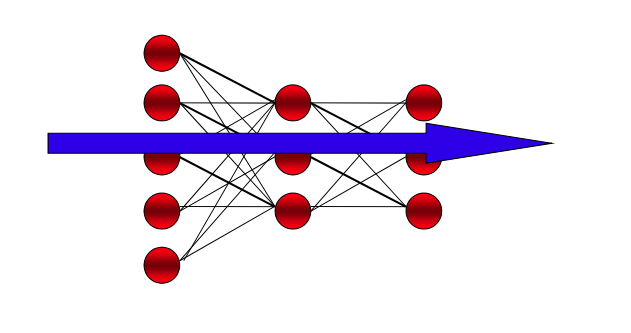
\includegraphics[width=0.8\textwidth]{bilder/forward_prop.png}
    \caption{The forward pass in backpropagation \cite{website:inf_4490_mlp}}
    \label{fig:forward_step}
\end{figure}

The backpropagation algorithm consists of two main steps. The first being the forward pass, which has the following structure illustrated in figure \ref{fig:forward_step}. After the input layer has received its inputs, the activations of the hidden nodes in the middle layer is calculated. Lastly the activations of the output nodes in the last layer is being calculated. 

\begin{figure}[ht]
    \centering
    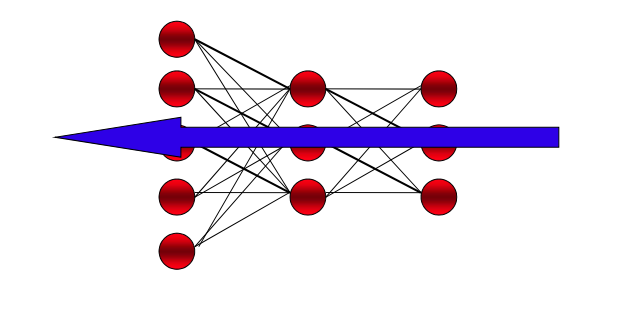
\includegraphics[width=0.8\textwidth]{bilder/backward_prop.png}
    \caption{The backward pass in backpropagation \cite{website:inf_4490_mlp}}
    \label{fig:backward_step}
\end{figure}

The second step in the backpropagation is called the backward pass, and is illustrated in figure \ref{fig:backward_step}. This step starts by calculating the output errors in the last layer, before it update the same layers weights. Then the error is being propagated backwards, and the hidden weights in the middle layer is updated. This process is repeated until the first layer is reached.
\subsection{Gradient descent learning and momentum}
When training the network with backpropagation, the goal is to minimizing the errors in the network. As described with the backward pass, after being calculated, the errors from the output layer are propagated backwards in the network. The tool being used is a form of gradient descent. 

\begin{equation}\label{eq:sum_of_error}
\begin{aligned}
E(w) = \frac{1}{2} \sum_{k}(t_k - y_k)^2 = \frac{1}{2}\sum_{k}(t_k - \sum_{i} \omega_{ik}x_i)^2
\end{aligned}
\end{equation}

It differentiate the sum-of squares error in equation \ref{eq:sum_of_error}, showed with the equation \ref{eq:gradient_descent}.  

\begin{equation}\label{eq:gradient_descent}
\begin{aligned}
\Delta\omega_{ik} = -\eta\frac{\delta E}{\delta \omega_{ik}}
\end{aligned}
\end{equation}

Even though gradient descent algorithm is a good method for finding the minimum value, it has a potential risk of getting stuck in a local minimum as visualized in figure \ref{fig:gradient_descent}.

\begin{figure}[ht]
    \centering
    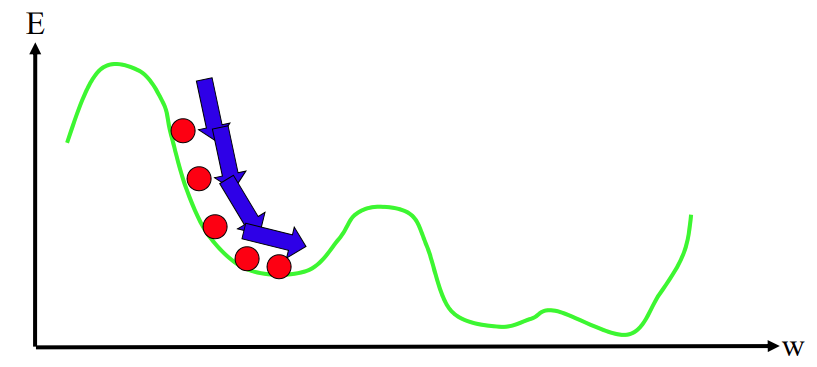
\includegraphics[width=0.8\textwidth]{bilder/gradient_descent.png}
    \caption{Gradient descent \cite{website:inf_4490_mlp}}
    \label{fig:gradient_descent}
\end{figure}

There is two alternatives to avoid being stuck in a local minimum. The first one is to initialize the training several times with random weights. The other method is to use momentum. If the gradient descent algorithm reaches a local minimum, the momentum keeps the algorithm going further uphill for a while, until the descending starts again and hopefully a global minimum will be found instead. Momentum is described mathematically in equation \ref{eq:momentum}. 

\begin{equation}\label{eq:momentum}
\begin{aligned}
w_{ij} \longleftarrow w_{ij} - \eta\Delta_j z_i+\alpha\Delta w^{t-1}_{ij}
\end{aligned}
\end{equation}

\subsection{Activation functions}
The task of an activation function is to decide whether a neuron should \textit{"fire"} or not. In other words, the activation function takes a number and performs a mathematically operation on it. There exist several activations functions, all with different pros and cons. The ones being used in this thesis will be covered here.
\subsubsection{The sigmoid function}
The sigmoid function was a historically often used activation function. It is mathematically described with equation \ref{eq:sigmoid}.
\begin{equation}\label{eq:sigmoid}
\begin{aligned}
\sigma(x) = \frac{1}{(1 + e^{-x})}
\end{aligned}
\end{equation}

The function transforms the input numbers into a range between 0-1 as shown in figure \ref{fig:sigmoid}. This means large negative numbers become 0, while large positive number become 1.

\begin{figure}[ht]
    \centering
    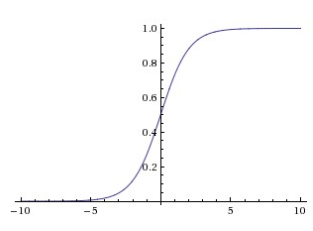
\includegraphics[width=0.6\textwidth]{bilder/sigmoid_function.png}
    \caption{Sigmoid activation function \cite{website:cs231n_activation_functions}}
    \label{fig:sigmoid}
\end{figure}

Nowadays the popularity of the the sigmoid function has decreased due to the following drawbacks:
\begin{itemize}
    \item \textit{Vanishing gradients at values close to 0 or 1}
    \item \textit{The neurons can be saturated if the initial weights are too large}
    \item \textit{The outputs are not zero-centered}
\end{itemize}

\subsubsection{The ReLu function}
The ReLu function (Rectified Linear Unit) has become increasingly more popular in the last few years. It is proven much faster than the sigmoid or tanh (which is a scaled sigmoid function) functions in a paper, due to its linear, non-saturating form \cite{website:relu}. 

\begin{equation}\label{eq:reLu}
\begin{aligned}
f(x) = max(0,x)
\end{aligned}
\end{equation}

\begin{equation}\label{eq:reLu_2}
\begin{aligned}
{f(x) = 
\begin{cases}
    0 & \text{for x < 0}  \\
    x & \text{for x $\geq$ 0}
\end{cases}}
\end{aligned}
\end{equation}

The ReLu function is described mathematically in two ways in this thesis, both being illustrated in equation \ref{eq:reLu} and equation \ref{eq:reLu_2} for a better understanding of the function.

\begin{figure}[ht]
    \centering
    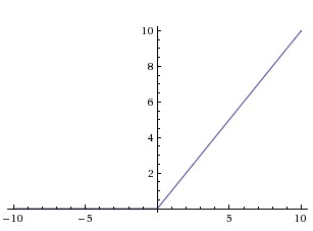
\includegraphics[width=0.6\textwidth]{bilder/relu_activation.png}
    \caption{Relu activation function \cite{website:cs231n_activation_functions}}
    \label{fig:relu}
\end{figure}

As illustrated in figure \ref{fig:relu} the ReLu activation is thresholded at zero. This makes ReLu a favored choice over the sigmoid/tanh functions. It is a less computational heavy method, because it does not have the exponential implementation. There is however one disadvantage using ReLu. The units can be fragile during training and as much as 40\% of the network may end up \textit{"dead"}. This can happen if a large gradient is flowing through the ReLu neuron. It may cause the neuron to update in such a way that the neuron never will activate on a data point again and end up \textit{"dead"}. With a proper learning rate (not too high), the problem tends to be avoided in most cases.

\subsection{Loss and optimizers}
The task of a loss function is to measure the distance between the predictions being made by the network and the actual ground truth. In this manner there can be computed a distance score, controlling how well the network did with its prediction \cite{Francois_Deep_learning_with_python}. This is illustrated in figure \ref{fig:loss_function}.

\begin{figure}[ht]
    \centering
    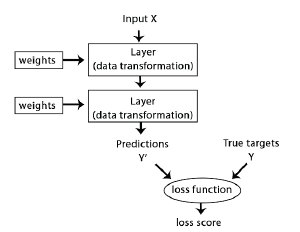
\includegraphics[width=0.6\textwidth]{bilder/loss_function.png}
    \caption{Loss function \cite{Francois_Deep_learning_with_python}}
    \label{fig:loss_function}
\end{figure}

The loss score computed by the loss function, is further being used as a feedback signal for adjusting the weights slightly. The weights are updated in a direction which lower the loss score, in order to make better future predictions. This is shown in figure \ref{fig:optimizers}. The job of adjusting the weights is executed by what is called an optimizer. The optimizer implements the backpropagation algorithm earlier described in this section \cite{Francois_Deep_learning_with_python}. 

\begin{figure}[ht]
    \centering
    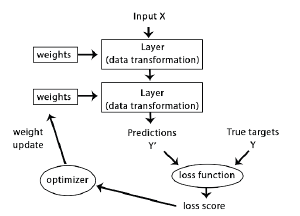
\includegraphics[width=0.6\textwidth]{bilder/optimizers.png}
    \caption{The visualization of an optimizer \cite{Francois_Deep_learning_with_python}}
    \label{fig:optimizers}
\end{figure}


\subsection{Regularization}
To avoid the term overfitting (explained in page 95 \& 96 \cite{Francois_Deep_learning_with_python}), the implementation of regularization will be helpful. Regularization refers to regulating the weights, by constraining them to only accept small values. It is implemented by adding a \textit{cost} to the loss function if it has too large weights. The cost comes in two different forms:

\begin{itemize}
    \item \textit{\textbf{L1 regularization}}
    \item \textit{\textbf{L2 regularization}}
\end{itemize}
Where \textit{L1 regularization} adds the costs proportionally to the absolute value of the weights coefficients, and \textit{L2 regularization} adds the costs proportionally to the square of the absolute value of the weights coefficients \cite{Francois_Deep_learning_with_python}. 
\newline
\newline
Another popular regularization method is \textit{dropout}, developed by Hinton and his students at the University of Toronto \cite{website:dropout}. It consists of randomly zeroing out (dropping out) a number of output features of the layer during training. The term \textit{"dropout rate"} refers to the fraction of the features which is being dropped out, and is usually put to a number between 0.2-0.5. When the algorithm is ready for testing, the output values are scaled down with a factor equal to the dropout rate instead of being dropped out. This is done in order to balance for the amount of more active units during testing. To use dropout as a regularization method is both very common and efficient \cite{Francois_Deep_learning_with_python}.   

\subsection{Convolutional neural networks}
A \ac{cnn} is a sub class of \ac{ann}. The main difference between a \ac{cnn} and an ordinary neural network is how the input is interpreted. In a \ac{cnn} the inputs is assumed to be images. 
\newline
\newline
Unlike a \ac{cnn}, an ordinary neural network with fully connected layers will keep all parameters connected from the input until the output. The \ac{cnn} with the use of convolutions, are able to reduce the numbers of parameters vastly from each layer while keeping the key features. This difference makes \ac{cnn} a much better tool for processing images, as images contains more parameters compared to most other form of inputs. 
\newline
\newline
The following example will demonstrate why it is necessary to reduce the parameters when processing images. Imagine an ordinary neural network with an image (width, height, depth) as an input. The size of the input is (200 x 200 x 3). This means the number of weights will become $224 * 224 * 3 = 150528$ weights. Adding more similar neurons, will escalate the number of parameters considerably, which then will result in an unnecessary overfitting and a poorly network.
\newline
\newline
The characteristics of a \ac{cnn} is described below, providing a general understanding how the parameters are being reduced and its unique features.
\subsubsection{Convolutional Layer}
Being the core building block of a \ac{cnn}, the convolutional layer does mostly of the computational heavy work necessary for the network to perform well. 
It is build up by learnable filters which slides through the whole input image bit by bit. Equation \ref{eq:conv} illustrates the general expression of a 1D convolution. Where $\omega$ is the filter being convolved with the input $f(x,y)$, providing the output $g(x,y)$. 

\begin{equation}\label{eq:conv}
\begin{aligned}
g(x,y) = \omega * f(x,y) = \sum_{s=-a}^{a}\sum_{t=-b}^{b}\omega(s,t)f(x-s,y-t)
\end{aligned}
\end{equation}

\begin{figure}[ht]
    \centering
    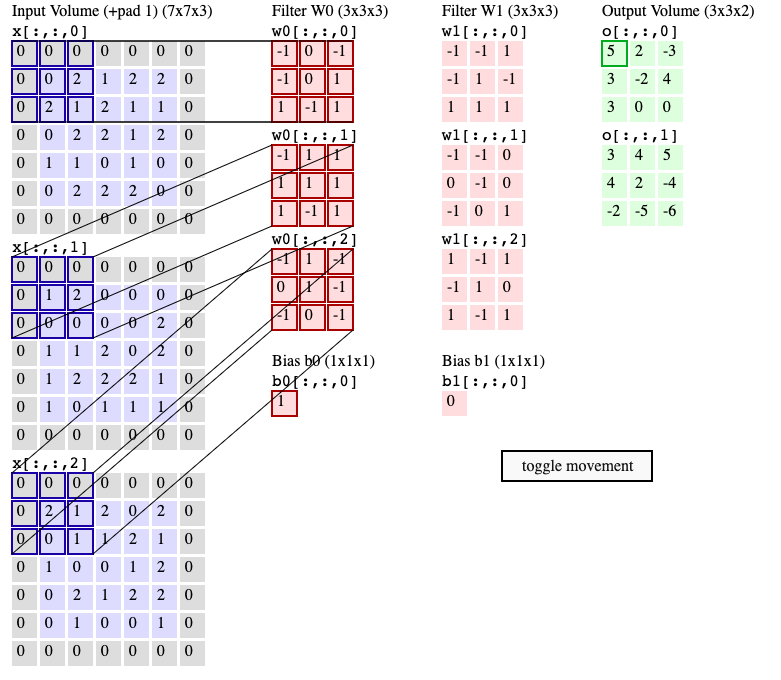
\includegraphics[width=0.8\textwidth]{bilder/conv2.png}
    \caption{3D Convolution step by step \cite{website:cs231n}}
    \label{fig:conv}
\end{figure}

To understand the process even better, the Stanford course \textit{"CS231n:  Convolutional  Neural  Networks  for  Visual Recognition"} has provided a intuitive visual model showing a 3D convolution explicitly in figure \ref{fig:conv}. This illustration consists of following parameters and configurations:

\begin{itemize}
    \item \textit{Input volume = (7x7x3)}
    \item \textit{Stride = 2}
    \item \textit{Number of zero padding = 1}
    \item \textit{Two weight filters = (3x3x3)}
    \item \textit{Two biases = (1x1x1)}
    \item \textit{Output volume = (3x3x2)}
\end{itemize}

Where the first weight filter $W0$ is sliding over each part of the input in its three channels. This gives the output volume o[:,:,0], while the convolving of weight filter $W1$ provides o[:,:,1]. The stride is set equal to two, which means the filter can slide in three positions both in $x$- and $y$-direction. This operation makes the output dimension into width and height equals to 3. The last dimension in the output volume is set by the amount of filters ($W0$ and $W1$) convolving over the input volume. The amount of chosen filters is a hyperparameter and decides the depth of the output. In this example there is two filters, which means the final output volume becomes (3x3x2). 
The implementation of zero padding helps us to control the spatial size of the output. It is also a hyperparameter and in this example it is set equal to one, which gives us the pad (marked in grey in figure \ref{fig:conv}) around the input volume filled with zeros. 
\newline
\newline
The equation to compute the spatial size of the output volume is illustrated in \ref{eq:output_conv}

\begin{equation}\label{eq:output_conv}
\begin{aligned}
O = \frac{(W - F + 2P)}{S}+1
\end{aligned}
\end{equation}

Where $O$ is the output volume. $W$ is the input volume, $F$ is the receptive field (the weight filter), $P$ being the amount of zero padding, and $S$ for the number of strides.
 
\subsubsection{Parameter sharing and local connectivity}
In contrary to ordinary neural networks, \ac{cnn} have neurons set up in three dimension. Width, height and depth. These neurons may have various levels of connectivity between the layers. The two concepts controlling and reducing the amount of connections between the neurons is called parameter sharing and local connectivity. As earlier described one of the main reason for the \ac{cnn} to out perform ordinary neural networks (when processing images), is its properties to reduce the amount of parameters while keeping key features. 
\newline
\newline
Parameter sharing means to share some weights and biases in order to control the number of parameters. This can be done with taking the assumption that if a feature is useful to calculate at a specific spatial location ($x_1$,$y_1$), it should be useful to compute it at a different location ($x_2$,$y_2$) as well. In practices that means constraining the neurons in each depth dimension to use same weights and bias. parameter sharing will greatly reduce the amount of total weights, and is an important contribute to make an efficient \ac{cnn}. 
\newline
\newline
Local connectivity connects each neuron only to a small region of the previous layers input. Unlike connecting the neurons to all the neurons from the previous layer as done in ordinary neural networks.
This small region is a hyperparameter, and is called the receptive field of the neuron. It is the same as the weight filter from the example above. The depth slice in the weight filter is always the same as the depth slice from the previous layers input. This means that we have local connections along width and height, and full connection along the depth of the input layer.

\subsection{Pooling layer}
Another method to reduce parameters is to add a max pool layer. Similarly to the convolution layer it contains a filter ($F$) and stride ($S$). 

\begin{figure}[ht]
    \centering
    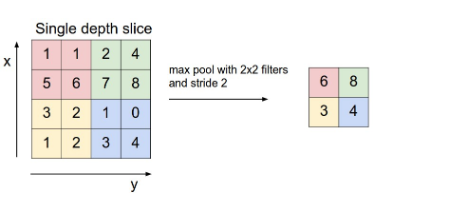
\includegraphics[width=0.8\textwidth]{bilder/max_pooling.png}
    \caption{Max pooling \cite{website:cs231n}}
    \label{fig:max_pooling}
\end{figure}

But as seen in figure \ref{fig:max_pooling}, the filter takes the max value in each frame instead of convolving through the input like the convolution layer does. The most common values in the max pooling layer is $F=$2 or 3, and $S=2$. Increasing those values will result in a destructive layer. It is a common practice to implement a max pool layer periodically between convolutional layers.

\section{Generating the ground truth labels}
There exist several good programs for generating labels for data sets. All with different pros and cons. The one being used for this thesis is a free program which offer offline annotation. It is called \textit{"labelme"}, and it can be installed directly from GitHub \cite{website:labelme}. The program is easy to learn and contains annotation examples in the GitHub folder. \textit{Labelme} has a clean programmed \ac{gui} regarding the working space, which is illustrated in figure \ref{fig:annotate}. 

\begin{figure}[ht]
    \centering
    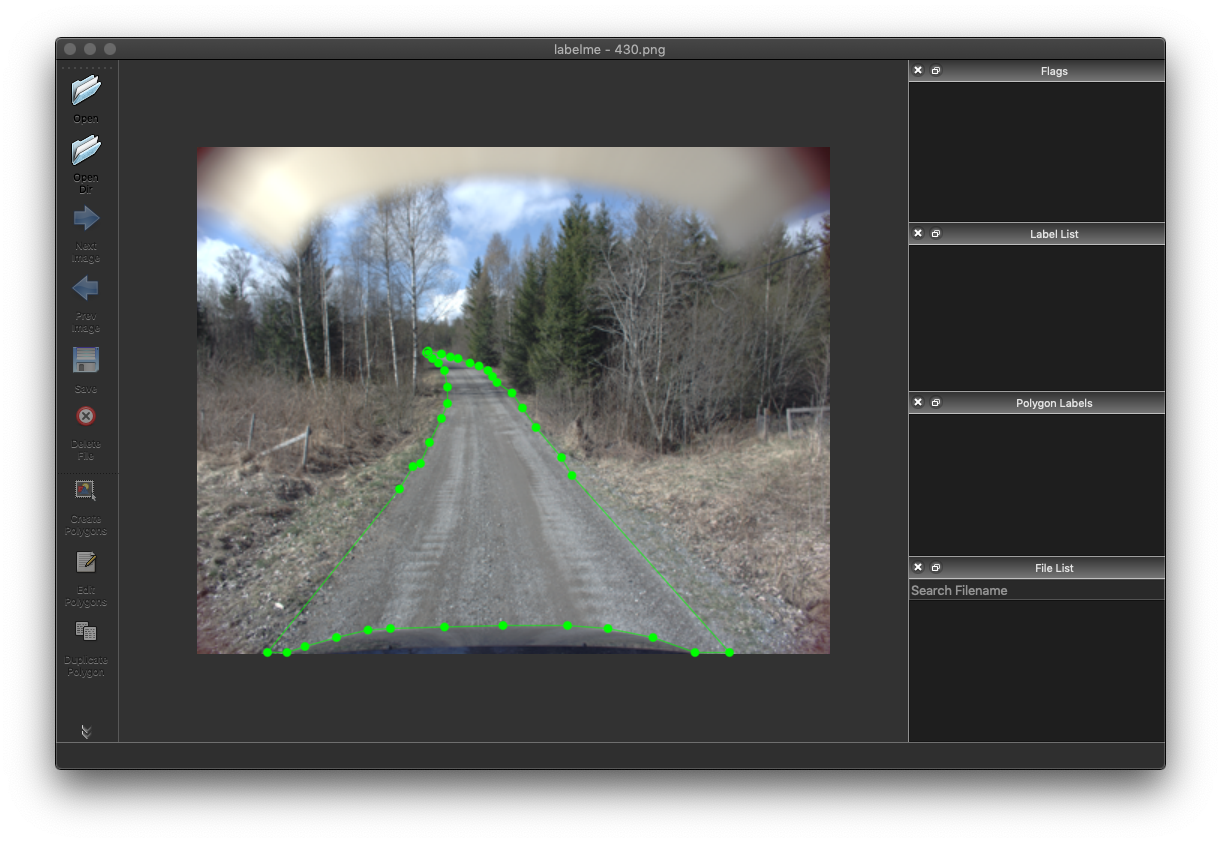
\includegraphics[width=0.8\textwidth]{bilder/annotating.png}
    \caption{Manually annotating an image with labelme}
    \label{fig:annotate}
\end{figure}

When the polygon is finished being drawn, another script is run, and the complete annotation ends up like in figure \ref{fig:finished_annotation}.  

\begin{figure}[ht]
    \centering
    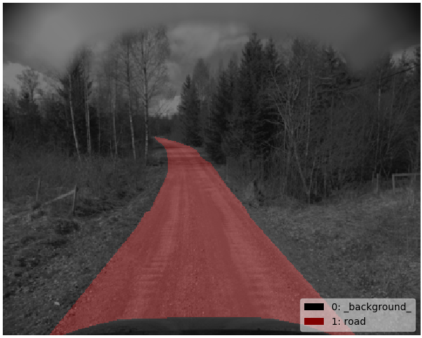
\includegraphics[width=0.6\textwidth]{bilder/label_viz.png}
    \caption{A complete annotation}
    \label{fig:finished_annotation}
\end{figure}

\chapter{Related works}
\section{U-net}

\begin{figure}[ht]
    \centering
    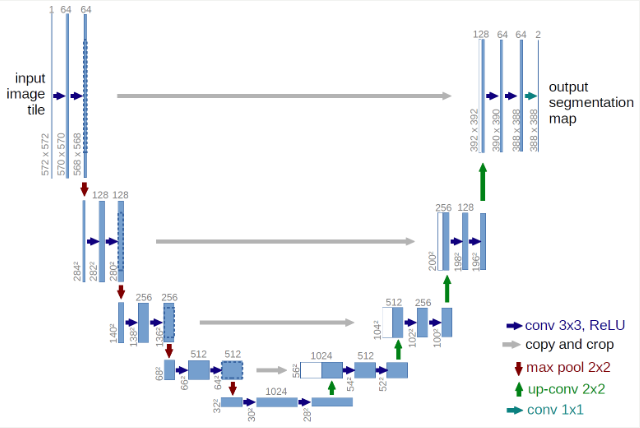
\includegraphics[width=0.8\textwidth]{bilder/u_net.png}
    \caption{The structure from the U-Net \cite{website:u_net}}
    \label{fig:u_net}
\end{figure}

\section{DeepLab}

\chapter{Method}
\section{Implementation}
\subsection{Annotation the training set}
When the images in this thesis has been annotated, only two classes were assigned each image. Class 0 to background, and class 1 to road.
\subsection{Keras}
Keras is a user-friendly \ac{dl} library developed in Python. It was originally made for researchers as way to do quick experimentation, with an easy implementation. Keras has quickly gained popularity among its users and is one of the most popular framework in \ac{dl} projects nowadays. The main reasons for the popularity is the user-friendliness and that Keras can run with the same code seamlessly on \ac{cpu} or \ac{gpu}\cite{Francois_Deep_learning_with_python}.
\subsection{Training, validation and testing data}

In order to have a successful implementation, the data set must be split into different parts. Either splitting the data set in training and test, or training, validation and test. The network should only train on the training set, then check accuracy on the validate set and predict values on the testing set. The validation- and test set should be data that the network never has seen before. There is a rule of thumb to split the data in training, validation and test set 60/20/20.  
\todo{skriv om sklearn biblioteket(i metode kap), og hvorfor det er viktig å splitte datasettet korrekt}
\subsection{The residual network}
\subsection{The sequential network}
\subsection{Tensorboard}
A handy way to gain control over the training, in order to tweak parameters and control the models accuracy, is using Tensorboard. Tensorboard is a visual tool developed by TensorFlow providing full overview of the training, while training. It is easy to set up in the terminal.
\begin{figure}[ht]
    \centering
    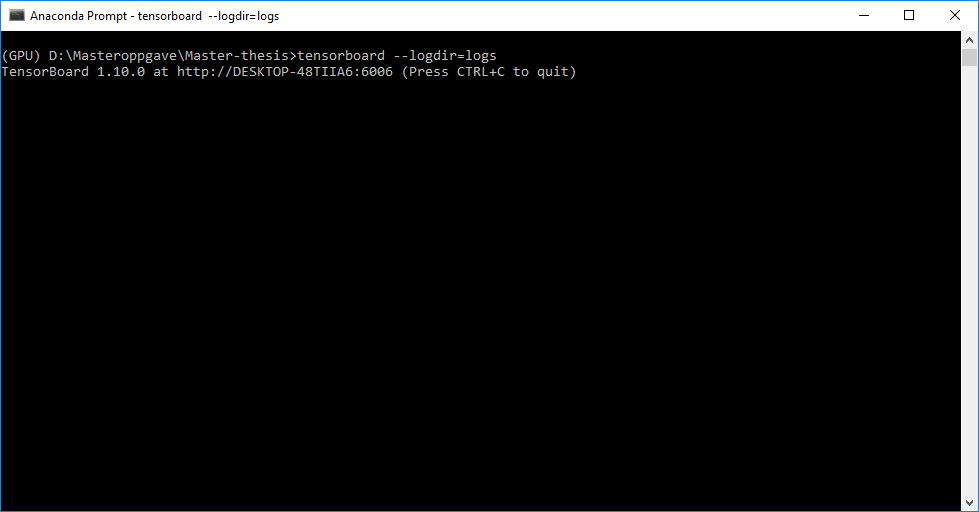
\includegraphics[width=0.8\textwidth]{bilder/tensorboard_anaconda_prompt.PNG}
    \caption{Initializing Tensorboard from terminal}
    \label{fig:tensorboard_anaconda_prompt}
\end{figure}
\newline
As illustrated in figure \ref{fig:tensorboard_anaconda_prompt} Tensorboard is up and running with the command \textit{< tensorboard --logdir=<log> >}. 
\newline
When using Tensorboard with Keras, there is necessary to use callbacks in the code. As stated by the Keras documentation on their website.
\newline
\newline
\textit{"A callback is a set of functions to be applied at given stages of the training procedure. You can use callbacks to get a view on internal states and statistics of the model during training. You can pass a list of callbacks (as the keyword argument callbacks) to the .fit() method of the Sequential or Model classes. The relevant methods of the callbacks will then be called at each stage of the training."}\cite{website:Keras_doc}. 
\newline
\newline
It is therefore possible with callbacks to decide by own specifications what to include and when to gain information during the training process.  
\begin{figure}[ht]
    \centering
    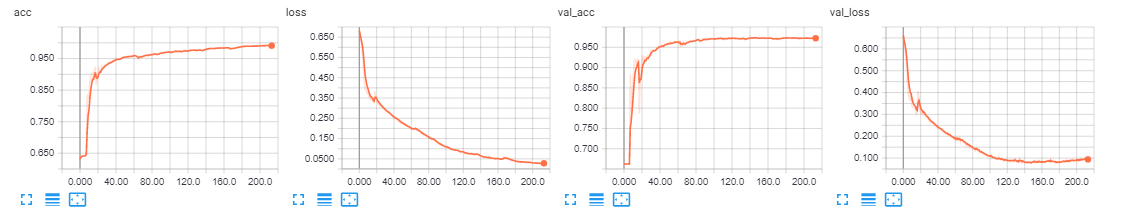
\includegraphics[width=1\textwidth]{bilder/tensorboard_acc_loss.PNG}
    \caption{Accuracy and loss for both training and validation visualized in Tensorboard}
    \label{fig:accuracy_loss}
\end{figure}
\newline
Two popular graphs used to check the quality of the \ac{dl} model is \textit{"accuracy"} and \textit{"loss"}, which are found under the section \textit{"SCALARS"}. 
\begin{figure}[ht]
    \centering
    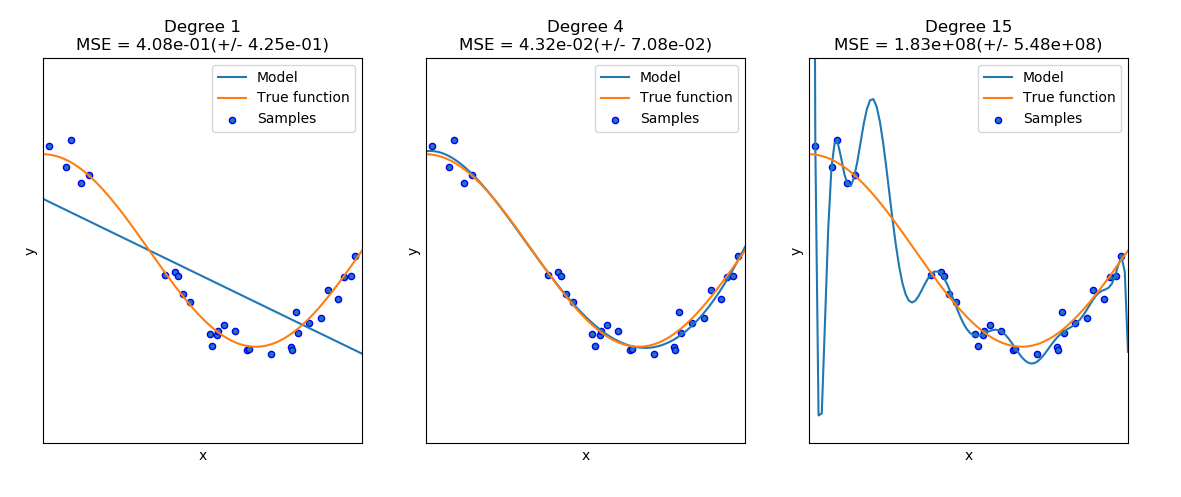
\includegraphics[width=1\textwidth]{bilder/overfitting_underfitting.png}
    \caption{Underfitting, perfect sampling and overfitting \cite{website:overfitting_underfitting}}
    \label{fig:overfitting_underfitting}
\end{figure}
To have the opportunity to visually see these graphs during training, is an advantage. This is due to the possibility of easily spotting errors like \textit{"overfitting"} or \textit{"underfitting"}, and if the accuracy in the model is fulfilling user expectations. Examples of underfitting from the left image, perfect sampling in the middle and overfitting in the right image, can be seen in figure \ref{fig:overfitting_underfitting}. As seen in figure \ref{fig:accuracy_loss} the accuracy and loss in both training and validation fulfil expectations. 
By observing that the loss function steadily decreases into a smooth curve indicates that there is neither \textit{"overfitting"} nor \textit{"underfitting"} in the model.

\begin{figure}[t!]
    \centering
    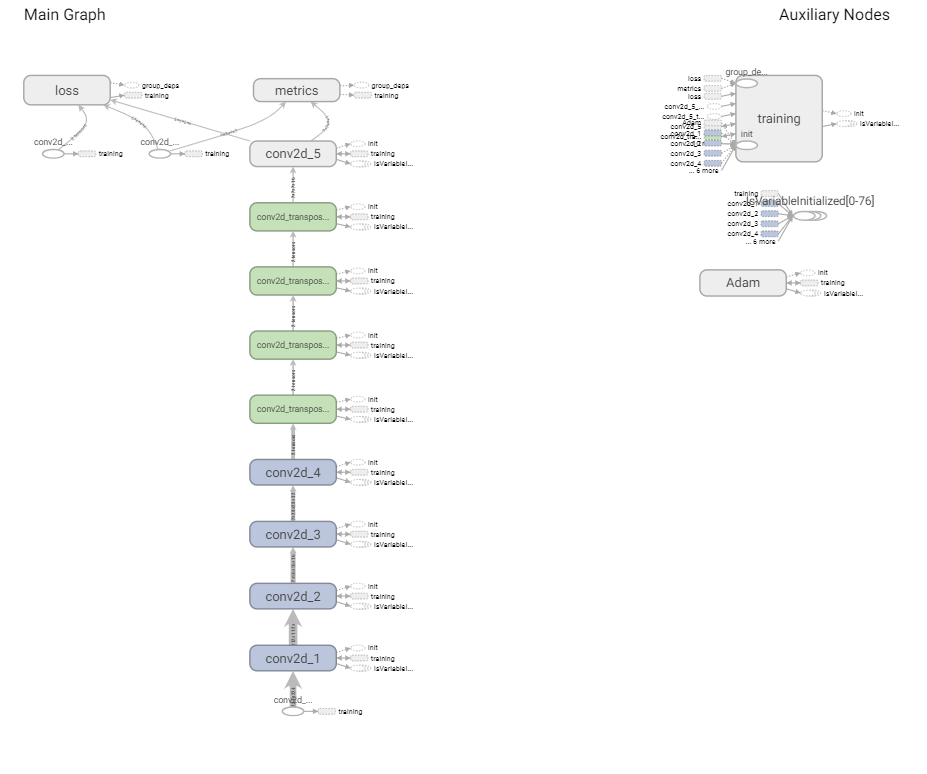
\includegraphics[width=0.8\textwidth]{bilder/tensorboard_graph.PNG}
    \caption{The model graph visualized in Tensorboard}
    \label{fig:graph}
\end{figure}
The other section in Tensorboard called \textit{"GRAPHS"} shows the model graph. Being able to see the layers, optimizer function and connections, helps the user see the whole model in a better perspective. There is possible to rename each layer in the model according to the user's own request. 
\section{Predictions}
After the network has updated the internal state well enough and learned the input and output, it can be fed new data it has never seen before. It will predict an output given the input of the new data, given the networks internal state.  
\subsection{Techniques from computer vision}
\subsubsection{Thresholding}
\subsubsection{CCA}
\subsubsection{Binary hole filling}

\chapter{Results}                     

\chapter{Discussion}

\chapter{Conclusion}



\backmatter{}
\printbibliography
\end{document}
